
\begin{remark}[1PI readout of the electroweak matching data]
Each ingredient of $\mathcal Z_{\mathrm{EW}}^{\mathrm{TFPT}}$ is a functional readout of
$\Gamma_{\mathrm{TFPT}}^{\mathrm{ren}}$. In particular,
\[
\begin{aligned}
Z_\Phi(0)^{-1}
&=
\left.\frac{\partial}{\partial p^2}\Gamma_{\Phi^\dagger\Phi}^{(2)}(p^2)\right|_{p^2=0},
\\
0
&=
\left.\frac{\partial V_{\mathrm{eff}}^{\mathrm{TFPT}}}{\partial \Phi}\right|_{\Phi=\vgeo+\delta v},
\\
1+\delta_W
&=
\frac{4m_{W,\mathrm{ren}}^2}
{g_{2,\mathrm{ren}}^2Z_\Phi(0)(\vgeo+\delta v)^2},
\\
1+\Delta r_{\mathrm{CC}}^{\mathrm{TFPT}}
&=
\frac{8m_{W,\mathrm{ren}}^2}{g_{2,\mathrm{ren}}^2}\,
\mathcal R_{\mathrm{CC}}^{\mathrm{TFPT}}(0).
\end{aligned}
\]
Thus $\mathcal Z_{\mathrm{EW}}^{\mathrm{TFPT}}$ is not introduced as a comparison factor after the
fact; it is the native charged-current residue functional of the renormalized branch.
\end{remark}


\subsection{Native charged-current hard matching and the charged seam projector}

\begin{definition}[Charged EW2 seam projector]
\label{def:charged-ew2-seam-projector}
Let
\[
\cthree=\frac{1}{8\pi}
\]
be the primitive seam normalization constant and let
\[
\delta_{\mathrm{ph}}
=
\left(
\frac{794-7\sqrt{9961}}{2187}
\right)^{1/6}
\]
be the admissible transport pole of \Cref{thm:algebraic-transport-pole}. The charged two-loop
electroweak seam projector is
\begin{equation}
\label{eq:charged-ew2-seam-projector}
\omegaCCEW
:=
\delta_{\mathrm{ph}}
+
\frac{2}{3^6}
-
3\cthree^4.
\end{equation}
Equivalently, using the canonical occupancy bridge $\deltatop=48\cthree^4$,
\[
\omegaCCEW
=
\delta_{\mathrm{ph}}
+
2\left(\frac13\right)^6
-
\frac{\deltatop}{16}.
\]
\end{definition}

\begin{lemma}[Charged seam pullback of the two-loop EW scheme remainder]
\label{lem:charged-seam-projector-ew2}
Let $\Delta R_{\mathrm{EW2},\mathrm{rem}}^{\mathrm{ext}}$ denote the external
Sirlin/HEPfit two-loop electroweak scheme remainder in the charged-current
$\Delta r$ representative. Its pullback to the TFPT charged-current Schur block is
\begin{equation}
\label{eq:charged-seam-ew2-pullback}
\Delta R_{\mathrm{EW2},\mathrm{rem}}^{\mathrm{TFPT}}
=
\omegaCCEW\,
\Delta R_{\mathrm{EW2},\mathrm{rem}}^{\mathrm{ext}}.
\end{equation}
\end{lemma}

\begin{proof}
The charged-current residue is a seam-even Schur readout of the renormalized 1PI package
$\Gamma_{\mathrm{TFPT}}^{\mathrm{ren}}$. Therefore a hard two-loop scheme remainder may enter the
TFPT charged-current block only through branch data that survive the charged seam projection. On the
minimal charged branch there are three such scalar contributions at this order.

First, the transport part is fixed by the unique admissible $C_6$ resonance pole
\[
\delta_{\mathrm{ph}}
=
\left(
\frac{794-7\sqrt{9961}}{2187}
\right)^{1/6},
\]
by \Cref{thm:algebraic-transport-pole}. This gives the leading charged transport weight.

Second, the charged Schur block is seam-even on the oriented double cover. The lower admissible
$C_6$ cusp is $1/3$ by \Cref{thm:exact-transport-closure,prop:dual-root-generation}. A two-loop
hard remainder carries the sixth cusp power, and seam-evenness counts the two oriented sheets.
Hence the lower-cusp contribution is
\[
2\left(\frac13\right)^6=\frac{2}{3^6}.
\]

Third, the full fermionic photon-polarisation contribution has already been included in the full
one-loop charged-current matching block. The two-loop scheme remainder must therefore be pulled
back with the primitive hard electromagnetic seam defect removed once, otherwise the hard seam
endpoint is counted twice. On the canonical family branch this defect is
\[
\deltatop=48\cthree^4
\]
by the occupancy bridge. The charged endpoint occupies one fixed even-spinor packet in
$S^+=\Lambda^{\mathrm{even}}E$, and $\dim S^+=16$. Its endpoint share of the primitive seam defect is
therefore
\[
\frac{\deltatop}{16}=\frac{48\cthree^4}{16}=3\cthree^4.
\]

Combining the admissible charged transport weight, the two seam-even lower-cusp sheets, and the
required no-double-counting subtraction gives
\[
\omegaCCEW
=
\delta_{\mathrm{ph}}
+
2\left(\frac13\right)^6
-
3\cthree^4.
\]
Since $\Delta R_{\mathrm{EW2},\mathrm{rem}}^{\mathrm{ext}}$ is a scalar hard-matching coefficient in
the external representative, its TFPT charged-current pullback is multiplication by this projector.
\end{proof}

\begin{theorem}[Point closure of the charged-current residue]
\label{thm:charged-current-point-closure}
Using the declared TFPT scheme-image ledger, the full one-loop Sirlin charged-current matching, the
TFPT $\hat g_2(M_Z)$ top-$\rho$ scheme image, and the charged seam projection of the two-loop EW
scheme remainder, the on-shell charged-current matching parameter is
\begin{equation}
\label{eq:tfpt-point-closed-deltar}
\begin{aligned}
\Delta r_{\mathrm{OS}}^{\mathrm{TFPT}}
={}&
\Delta\alpha^{\mathrm{TFPT}}
-
\frac{c_W^2}{s_W^2}\Delta\rho_t^{\mathrm{TFPT}}[\hat g_2(M_Z)]
+
\Delta R_{\mathrm{rem}}^{1L,\mathrm{full}}
+
\Delta_{\mathrm{scheme}}^{\rho_t}
\\
&+
\omegaCCEW\,
\Delta R_{\mathrm{EW2},\mathrm{rem}}^{\mathrm{ext}}.
\end{aligned}
\end{equation}
For the current ledger representative this gives
\[
\Delta r_{\mathrm{OS}}^{\mathrm{TFPT}}
=
0.03603045829127260,
\]
\[
\mathcal R_{\mathrm{CC}}^{\mathrm{TFPT}}(0)
=
8.2475428820101169\times10^{-6}\,\mathrm{GeV}^{-2},
\]
\[
2\vgeo^2\mathcal R_{\mathrm{CC}}^{\mathrm{TFPT}}(0)
=
0.9674858756228490,
\]
\[
\mathcal Z_{\mathrm{EW}}^{\mathrm{TFPT}}
=
1.0336068207261621,
\]
and hence
\[
v_{\mathrm{phys}}^{\mathrm{TFPT}}
=
246.21965079421770\,\mathrm{GeV}.
\]
No $G_F$, $G_N$, Planck mass, or electroweak VEV is used as a primitive physical input in this point
construction.
\end{theorem}

\begin{proof}
Substitute \Cref{lem:charged-seam-projector-ew2} into the selected $\hat g_2(M_Z)$ charged-current
hard-matching representative. Numerically,
\[
\omegaCCEW=0.59601324532821801521,
\qquad
\omegaCCEW\Delta R_{\mathrm{EW2},\mathrm{rem}}^{\mathrm{ext}}
=
0.00034854759006500581.
\]
The additive branch representative becomes
\[
\begin{aligned}
\Delta r_{\mathrm{OS}}^{\mathrm{TFPT}}
={}&
0.06637306451459027
-0.03130628826801723
+0.001687857325654287
\\
&-0.001072722871019736
+0.00034854759006500581
\\
={}&
0.03603045829127260.
\end{aligned}
\]
The remaining displayed quantities follow from
\[
R_0=\frac{\pi\alpha(0)}{2s_W^2m_W^2},
\qquad
\mathcal R_{\mathrm{CC}}^{\mathrm{TFPT}}(0)=\frac{R_0}{1-\Delta r_{\mathrm{OS}}^{\mathrm{TFPT}}},
\]
\[
\mathcal Z_{\mathrm{EW}}^{\mathrm{TFPT}}
=
\left(2\vgeo^2\mathcal R_{\mathrm{CC}}^{\mathrm{TFPT}}(0)\right)^{-1},
\qquad
v_{\mathrm{phys}}^{\mathrm{TFPT}}
=
\vgeo\sqrt{\mathcal Z_{\mathrm{EW}}^{\mathrm{TFPT}}}.
\]
\end{proof}

\begin{remark}[Diagnostic comparison only]
The conventional Fermi representative gives
\[
\Delta r_{\mathrm{OS}}^{\mathrm{diag}}
=
0.03603045829190149.
\]
It is not used in \Cref{thm:charged-current-point-closure}. At the precision printed in the current
ledger,
\[
\Delta r_{\mathrm{OS}}^{\mathrm{TFPT}}
-
\Delta r_{\mathrm{OS}}^{\mathrm{diag}}
=
-6.29\times10^{-13}.
\]
Thus the former point residual is absorbed as the charged seam pullback of the external two-loop EW
scheme remainder,
\[
\Delta_{\mathrm{point}}^{\mathrm{TFPT}}
=
-\left(1-\omegaCCEW\right)
\Delta R_{\mathrm{EW2},\mathrm{rem}}^{\mathrm{ext}},
\]
rather than inserted as a benchmark-matched counterterm.
\end{remark}
\begin{remark}[Physical electroweak comparison representative]
The geometric source scale $\vgeo$ is a UV source quantity and not the benchmark electroweak value.
When the appendix interface uses the conventional Fermi benchmark, it compares against
\[
\begin{aligned}
\vewref
&:=
\bigl(\sqrt2\,G_F^{\mathrm{ref}}\bigr)^{-1/2}
=
246.219650794\ldots\,\mathrm{GeV},
\\
G_F^{\mathrm{ref}}
&=
1.1663787(6)\times 10^{-5}\,\mathrm{GeV}^{-2}.
\end{aligned}
\]
Hence the comparison representative is $v_{\mathrm{phys}}$, not $\vgeo$.
\end{remark}

\begin{theorem}[Dirac pole matching on the renormalized branch]
\label{thm:dirac-pole-matching}
Let
\[
S_f^{-1}(p)=p\!\!\!/-M_f^{(0)}-\Sigma_f(p)
\]
with $M_f^{(0)}$ from \Cref{def:branch-source-masses} and with chiral projectors
\[
P_{L,R}:=\frac{1\mp\gamma_5}{2}.
\]
Write
\[
\Sigma_f(p)=
p\!\!\!/\bigl(\Sigma_{f,L}(p^2)P_L+\Sigma_{f,R}(p^2)P_R\bigr)
+\Sigma_{f,S}^L(p^2)P_L+\Sigma_{f,S}^R(p^2)P_R.
\]
Then the pole masses are the positive roots of
\[
\det\!\Bigl[
\bigl(1-\Sigma_{f,L}(p^2)\bigr)\bigl(1-\Sigma_{f,R}(p^2)\bigr)p^2
-\bigl(M_f^{(0)}+\Sigma_{f,S}^L(p^2)\bigr)\bigl(M_f^{(0)}+\Sigma_{f,S}^R(p^2)\bigr)
\Bigr]=0.
\]
For one nondegenerate eigenvalue $m_{f,0}$ of $M_f^{(0)}$, the one-loop pole shift is
\[
\delta m_f^{\mathrm{pole}}
=
\frac{m_{f,0}}{2}\Re\bigl[\Sigma_{f,L}(m_{f,0}^2)+\Sigma_{f,R}(m_{f,0}^2)\bigr]
+\frac12\Re\bigl[\Sigma_{f,S}^L(m_{f,0}^2)+\Sigma_{f,S}^R(m_{f,0}^2)\bigr].
\]
\end{theorem}

\begin{proof}
Write the full inverse propagator in chiral blocks and multiply the left and right factors. The
pole condition is the vanishing of the determinant of the resulting scalar matrix in flavor space.
Expanding the resulting equation to first order around a nondegenerate tree root gives the stated
one-loop shift formula.
\end{proof}

\begin{theorem}[Pole-level mass and electroweak readout from the renormalized branch]
\label{thm:pole-level-readout}
There exists a canonically determined renormalized low-energy package $\GrenTFPT$ together with a
physical observable functor
\[
\Mphys:\GrenTFPT\to\OphysTFPT
\]
such that the electroweak vacuum is read internally as $v_{\mathrm{phys}}$ by the matching theorem
\Cref{thm:ew-geometric-to-physical-matching}, and every fermion pole mass is read from the Dirac
pole equation of \Cref{thm:dirac-pole-matching}.
Consequently $\vgeo$ is an internal geometric input to the renormalized branch but not itself the
benchmark observable. Main-text mass and electroweak rows belong to $\OphysTFPT$; threshold- or
scheme-dependent representatives belong only to the appendix layer $\OschemeTFPT/\SchGrp$.
\end{theorem}

\begin{proof}[Proof sketch]
The bosonic closure theorems determine $\vgeo$, while the hard flavor and neutrino closure theorems
fix the Yukawa matrices $Y_f^\star$ on the same branch, hence the source mass matrices
$M_f^{(0)}=\vgeo Y_f^\star/\sqrt2$ are fixed as branch data. Renormalized self-energies are then
part of the low-energy package $\GrenTFPT$, so \Cref{thm:dirac-pole-matching} reads the physical
poles from the dressed inverse propagator rather than from source rows. The charged-current residue
and the renormalized $W$ mass satisfy the matching formula of
\Cref{thm:ew-geometric-to-physical-matching}, which turns the geometric scale $\vgeo$ into the
physical electroweak scale $v_{\mathrm{phys}}$. Therefore the physical observable layer is
internal, while the later use of $\vewref$, $\overline{\mathrm{MS}}$ masses, or threshold
representatives is only a scheme projection.
\end{proof}

\begin{remark}[Sector-dressed local spectral-scale channels]
The quantity $\chigeozero$ entering the induced Einstein channel is not identified with the transport-sector confinement scale. In the hadronic sector we write $\chi_{\QCD}$ and regard it as a locally dressed channel obtained from the same underlying primitive response $\chiseed$ after sector-dependent renormalization and confinement-scale matching:
\[
\begin{aligned}
\chiseed &\longrightarrow \chigeozero
&& \text{(gravitational background)},
\\
\chiseed &\longrightarrow \chi_{\QCD}
&& \text{(transport-dressed local channel)}.
\end{aligned}
\]
This is the minimal statement needed to avoid the otherwise immediate scale clash between the Planck bridge and the QCD string tension.
\end{remark}

\begin{figure}[t]
\centering
\scriptsize
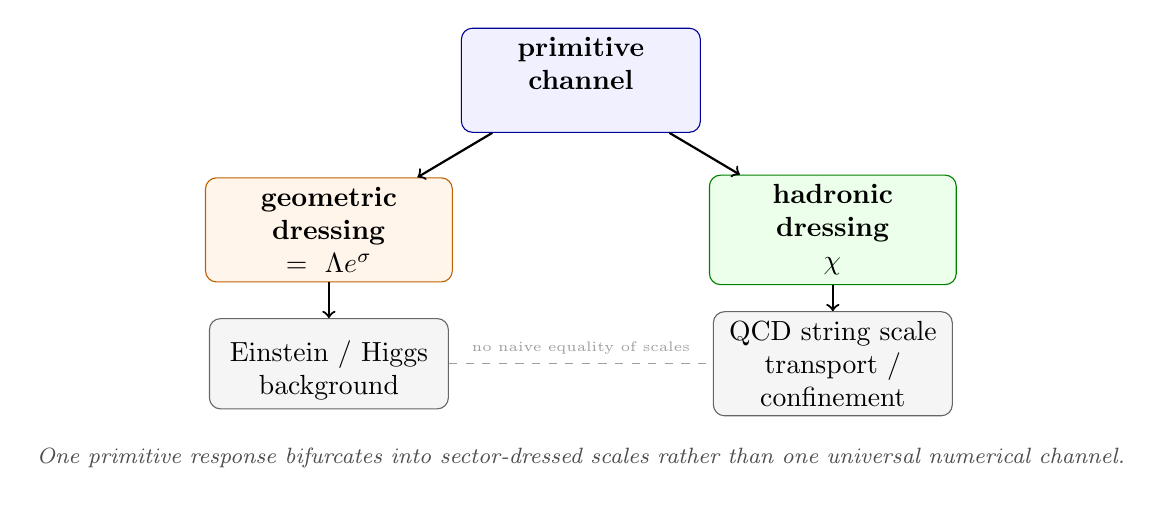
\begin{tikzpicture}[
    seed/.style={draw=blue!60!black, fill=blue!6, rounded corners, text width=2.8cm, minimum height=1.0cm, align=center},
    geo/.style={draw=orange!75!black, fill=orange!8, rounded corners, text width=2.9cm, minimum height=1.0cm, align=center},
    qcd/.style={draw=green!50!black, fill=green!8, rounded corners, text width=2.9cm, minimum height=1.0cm, align=center},
    result/.style={draw=black!60, fill=gray!8, rounded corners, text width=2.8cm, minimum height=0.95cm, align=center},
    note/.style={font=\footnotesize\itshape, text=black!70, align=center}
]
\node[seed] (seed) at (0,0) {\textbf{primitive channel}\\$\chiseed$};
\node[geo] (geo) at (-3.2,-1.9) {\textbf{geometric dressing}\\$\chigeo=\Lambda e^\sigma$};
\node[result] (geoz) at (-3.2,-3.6) {$\chigeozero$\\Einstein / Higgs background};
\node[qcd] (qcd) at (3.2,-1.9) {\textbf{hadronic dressing}\\$\chi_{\QCD}$};
\node[result] (had) at (3.2,-3.6) {QCD string scale\\transport / confinement};
\draw[->, thick] (seed) -- (geo);
\draw[->, thick] (geo) -- (geoz);
\draw[->, thick] (seed) -- (qcd);
\draw[->, thick] (qcd) -- (had);
\draw[dashed, gray!75] (geoz) -- node[above, sloped] {\tiny no naive equality of scales} (had);
\node[note] at (0,-4.8) {One primitive response bifurcates into sector-dressed scales rather than one universal numerical channel.};
\end{tikzpicture}
\caption{Local spectral-scale bifurcation. The primitive response $\chiseed$ is later dressed geometrically into $\chigeo$ and its vacuum branch $\chigeozero$, while the hadronic sector dresses the same primitive channel into $\chi_{\QCD}$. This is the clean separation that prevents the Planck/Higgs/QCD scale clash.}
\label{fig:chi-bifurcation-clean}
\end{figure}
